\chapter{Randomness Quality of CIPRNGs}
\label{Statistical Tests for Randomness}
\minitoc

In this chapter, for having comparison criteria, some classical PRNGs are evaluated by the statistical tests introduced in Section~\ref{Some famous statistical tests of random number generators}, namely the NIST, DieHARD, Comparative tests, and TestU01 test suites.
Regarding these results, we will be able to easily verify the improvements of mixing
such generators using chaotic iterations. Statistical performances of the CIPRNG
versions 3 and 4 are then given in a second part of this chapter. 
Finally four versions of CIPRNGs are assembled together, and a 
comprehensive comparison among them is produced using the aforementioned tests 
(for the sake of fairness, all the CIPRNGs have received two XORshifts as
inputted generators). 
These results have been formerly published in~\cite{bfg12a:ip, bfgw11:ij, bfgw11:ip}.

\section{Test results for some PRNGs}
We present in this section the scores obtained by four well known PRNGs
against the usual batteries of tests. These generators are respectively
the BBS, Logistic, XORshift, and ISAAC ones (details for these
generators have been given in Section~\ref{The generation of pseudorandom sequence}).

%\subsection{NIST results}
\label{for nist}

Table~\ref{The passing1} contains the $\mathbb{P}_T$ values 
corresponding to the test results of sequences from BBS, Logistic map, XORshift, and ISAAC 
respectively. 
We can see that, except for ISAAC, all the proposed generators failed
in passing the NIST battery ($\mathbb{P}_T$ values should be $\in \llbracket 0, 1 \rrbracket$). Results are particularly bad for the BBS
generator, although this PRNG is known to be cryptographically secure.
It is not contradictory, as these bad scores are due to the small prime 
numbers that have been used here as parameters of this PRNG.


\begin{table}
\renewcommand{\arraystretch}{1.3}
\caption{NIST SP 800-22 test results ($\mathbb{P}_T$)}
\label{The passing1}
\centering
\begin{tabular}{lcccc}
\toprule
Test name & BBS &Logistic& XORshift& ISAAC\\ 

Frequency (Monobit) Test 			&0.32435	&0.53414		&0.14532		&0.67868 \\ 
Frequency Test within a Block			&0.00000	&0.00275		&0.45593		&0.10252 \\ 
Runs Test 					&0.00000	&0.00000		&0.21330		&0.69931\\ 
Longest Run of Ones in a Block Test 		&0.00000	&0.08051		&0.28966		&0.43727 \\
Binary Matrix Rank Test 			&0.00000	&0.67868		&0.00000		&0.89776\\ 
Discrete Fourier Transform (Spectral) Test	&0.00000	&0.57490		&0.00535		&0.51412 \\ 
Non-overlapping Template Matching Test* 	&0.00000	&0.28468		&0.50365		&0.55515\\ 
Overlapping Template Matching Test 		&0.00000	&0.10879		&0.86769		&0.63711\\ 
Universal Statistical Test 			&0.00000	&0.02054		&0.27570		&0.69931 \\ 
Linear Complexity Test		        	&0.04335	&0.79813		&0.92407		&0.03756\\ 
Serial Test* (m=10) 				&0.00000	&0.41542		&0.75792		&0.32681 \\ 
Approximate Entropy Test (m=10) 		&0.00000	&0.02054		&0.41902		&0.30412\\ 
Cumulative Sums (Cusum) Test* 			&0.00000	&0.60617		&0.81154		&0.36786\\ 
Random Excursions Test* 			&0.00000	&0.53342		&0.41923		&0.50711 \\ 
Random Excursions Variant Test* 		&0.00000	&0.28507		&0.52833		&0.40930\\ \hline
Success 					&2/15 	&14/15		&14/15			&15/15 \\ 
\bottomrule
\end{tabular}
\end{table}

%\subsection{DieHARD results}
\label{Subsec:DieHARD}

Table~\ref{Results of DieHARD battery} contains, for its part, 
the results derived from applying the DieHARD battery of 
tests to the four generators considered in this section.
Another time, ISAAC is the sole generator able to pass the
whole battery, whereas the logistic map and the XORshift
generators present correct results. BBS, for its part, shows
another time a very bad statistical profile.

\begin{tiny}
\begin{table}[!t]
\renewcommand{\arraystretch}{1.3}
\caption{Results of DieHARD battery of tests}
\label{Results of DieHARD battery}
\centering
\begin{tabular}{llcccc} \toprule
No. &Test name &BBS &Logistic& XORshift& ISAAC\\
1 & Overlapping Sum &Pass&Pass &Pass&Pass\\
2 & Runs Up 1 &Pass & Pass &Pass&Pass\\
&Runs Down 1 &Pass &Pass &Pass&Pass\\
&Runs Up 2 &Pass &Pass &Pass&Pass\\
&Runs Down 2 &Pass & Pass &Pass&Pass\\
3 & 3D Spheres &Fail &Pass &Pass&Pass\\
4 & Parking Lot &Fail &Pass &Pass&Pass\\
5 & Birthday Spacing &Fail &Pass &Pass&Pass\\
6 & Count the ones 1 &Fail &Pass &Fail&Pass\\
7 &Binary Rank $6 \times 8$ &Fail & Pass &Pass&Pass\\
8 &Binary Rank $31 \times 31$ &Fail &Pass &Fail&Pass\\
9 &Binary Rank $32 \times 32$ &Fail &Fail &Fail&Pass\\
10 &Count the ones 2 &Fail &Pass&Pass&Pass \\
11 &Bit Stream &Fail &Pass&Pass&Pass \\
12 &Craps Wins &Fail &Pass&Pass&Pass \\
&Throws &Fail &Pass&Pass&Pass\\
13 &Minimum Distance &Fail &Pass &Pass&Pass\\
14 &Overlapping Perm. &Fail&Pass &Pass&Pass\\
15 &Squeeze &Fail &Pass &Pass&Pass \\
16 &OPSO &Fail &Pass &Pass&Pass \\
17 &OQSO &Fail &Pass &Pass&Pass \\
18 &DNA &Fail &Fail &Pass &Pass\\
&Number of tests passed &2&16 &15&18 \\ \bottomrule
\end{tabular}
\end{table}
\end{tiny}

%\subsection{Comparative test parameters}



\begin{table}[!t]
\renewcommand{\arraystretch}{1.3}
\caption{Comparative test parameters with a $10^7$ bits sequence}
\label{Comparison3}
\centering
\begin{tabular}{lccccc}
 \toprule
Method			&Threshold values 	 &BBS		&Logistic	& XORshift	& ISAAC\\
Monobit			&3.8415			&0.3485&0.1280		&1.7053		&0.1401\\ \hline
Serial		&5.9915 		&2.0079	 &0.1302		&2.1466		&0.1430\\ \hline
Poker			&316.9194 		&387.7216 	&240.2893	&248.9318	&236.8670\\ \hline
Runs 			&55.0027		&33.2067	&26.5667	&18.0087	&34.1273 \\ \hline
Autocorrelation		&1.6449			&-0.7603	& 0.0373	&0.5099 	&-2.1712\\ 
\bottomrule
\end{tabular}
\end{table}

In Table~\ref{Comparison3} is given another comparison of the BBS,
Logistic map, XORshift, and ISAAC generators using the comparative test 
parameters previously introduced, BBS is the only one generator which can't pass.
Finally, Table~\ref{TestU011} gives the results derived from applying the 
TestU01 battery to these PRNGs.
\begin{table}[!t]
\renewcommand{\arraystretch}{1.3}
\caption{TestU01 Statistical Test}
\label{TestU011}
\centering
\begin{tabular}{lcccccc}
\toprule
Test name &Battery&Parameters &BBS& Logistic 		& XORshift	& ISAAC\\
Rabbit 				&$32\times10^9$ bits	&38 &26	&21	 	&14	&0	 \\
Alphabit 			&$32\times10^9$ bits	&17 &9	&16 		&9	&0	 \\
Pseudo DieHARD 			&Standard		&126 &8	&0 	 	&2	&0	\\
FIPS\_140\_2 			&Standard		&16&0	&0 		&0	&0	\\
Small Crush 			&Standard		&15 &10	&4 		&5	&0	 \\
Crush 				&Standard		&144 &117	&95 		&57	&0	 \\
Big Crush 			&Standard		&160 &134	&125 	 	&55	&0	 \\ \hline
Number of failures 		& 			&516 &304	&261 	 	&146	&0	 \\
\bottomrule
\end{tabular}
\end{table}



%\subsection{Conclusion}
From the results shown in the four tables, statistical quality of each generator 
considered in this section can be basically deduced. 
BBS used in our conditions is not able to
produce reasonable sequences, the bad scores of these tests mainly relates to its too small period value. 
For the logistic map, it sounds better than BBS. However, this generator only successfully pass the comparative parameters tests.
Furthermore, its speed is far from dominating the comparison. 
XORshift failed to succeed the Binary Matrix Rank Test (NIST). 
This test focuses on the rank of disjoint 
sub-matrices extracted from the entire sequence. 
Note that this 
test also appears in the DieHARD battery.  
Such results mean that the 
null hypothesis $H_0$ must be rejected for these two bit streams, where $H_0$ is: ``for each integer $t>0$, the vector $(u_0 , ..., u_{t-1})$ is uniformly 
distributed over the $t$-dimensional unit cube $[0, 1]^t$''.
Finally, ISAAC plays best in all.

\section{Test results and comparative analysis for the CIPRNG version 3}
%\subsection{Results of NIST}
\label{Results of NISTfor Version 3 CI}
 
The generator version 3 
of the CIPRNG family is based on a 
Lookup table (LUT).
We test it here with the parameter $N$
equal to $4$.
We can conclude from Table~\ref{The passing for Version 3 LUT CI} that, except for the mixture of BBS and XORshift, all 
possible couples have successfully passed the NIST statistical test suite. The statistic of inputed XORshift and Logistic map are improved, and there is no reduction for ISAAC.
Remark that the use of BBS, having poor statistical performances, leads to outputs of LUT-1 not very uniformly distributed. 

\begin{table}
\renewcommand{\arraystretch}{1.3}
\caption{NIST SP 800-22 test results ($\mathbb{P}_T$) for Version 3 LUT CI algorithms}
\label{The passing for Version 3 LUT CI}
\centering
\begin{tabular}{lccc}
\toprule
\multirow{4}*{Test name} & \multicolumn{3}{c}{Version 3 LUT CI}\\
& XORshift& ISAAC &BBS\\ 
& +& + & + \\ 
& XORshift& XORshift&XORshift\\\cmidrule(r){2-4}
Frequency (Monobit) Test 			&0.32435 		&0.33171		&0.00000 \\ 
Frequency Test within a Block			&0.85643		&0.42327		&0.13233\\ 
Runs Test 					&0.11623		&0.31908		&0.00000\\ 
Longest Run of Ones in a Block Test 		&0.74254		&0.86688		&0.00000 \\
Binary Matrix Rank Test 			&0.23224		&0.88317		&0.90311\\ 
Discrete Fourier Transform (Spectral) Test	&0.12316		&0.34578		&0.59559 \\ 
Non-overlapping Template Matching Test* 	&0.43295		&0.32637		&0.00000 \\ 
Overlapping Template Matching Test 		&0.31472		&0.55915		&0.00000\\ 
Universal Statistical Test 			&0.37864		&0.24925		&0.06282 \\ 
Linear Complexity Test			&0.65723		&0.31793		&0.94630 \\ 
Serial Test* (m=10) 				&0.43532		&0.55190		&0.00000 \\ 
Approximate Entropy Test (m=10) 		&0.34254		&0.12482		&0.00000\\ 
Cumulative Sums (Cusum) Test* 			&0.11272		&0.04065		&0.14139 \\ 
Random Excursions Test* 			&0.02003		&0.32275		&0.34625 \\ 
Random Excursions Variant Test* 		&0.43554		&0.234294		&0.55048\\ \hline
Success 					& 15/15			&15/15		&8/15	 \\ 
\bottomrule
\end{tabular}
\end{table}

%\subsection{Results of Diehard}
Table~\ref{Results of DieHARD battery of tests for Version 3 LUT CI algorithms} gives 
the results derived from applying the DieHARD battery of tests to the PRNGs considered in this chapter. 
For the same reasons as in the NIST test suite's results, the CIPRNG constituted by the mixture of 
BBS and XORshift is not able to pass all the DieHARD battery.

\begin{tiny}
\begin{table}
\renewcommand{\arraystretch}{1.3}
\caption{Results of DieHARD battery of tests for Version 3 LUT CI algorithms ($\mathsf{N}=4$)}
\label{Results of DieHARD battery of tests for Version 3 LUT CI algorithms}
\centering
\begin{tabular}{llcccc} \toprule
\multirow{3}*{No.} &\multirow{3}*{Test name} & \multicolumn{4}{c}{Version 3 CI}\\
&&Logistic& XORshift& ISAAC&BBS \\ 
&&+& +& + & + \\ 
&&Logistic& XORshift& XORshift&XORshift \\ \cmidrule(r){3-6}
1 & Overlapping Sum &Pass &Pass &Pass&Fail\\
2 & Runs Up 1 &Pass & Pass &Pass&Pass\\
&Runs Down 1 &Pass &Pass &Pass&Pass\\
&Runs Up 2 & Pass &Pass &Pass&Pass\\
&Runs Down 2 &Pass & Pass &Pass&Pass\\
3 & 3D Spheres &Pass &Pass &Pass&Fail\\
4 & Parking Lot &Pass &Pass &Pass&Pass\\
5 & Birthday Spacing &Pass &Pass &Pass&Fail\\
6 & Count the ones 1 &Pass &Pass &Pass&Fail\\
7 &Binary Rank $6 \times 8$ &Pass & Pass &Pass&Pass\\
8 &Binary Rank $31 \times 31$ &Pass &Pass &Pass&Fail\\
9 &Binary Rank $32 \times 32$ &Pass &Pass &Pass&Fail\\
10 &Count the ones 2 &Pass &Pass&Pass&Fail \\
11 &Bit Stream &Pass &Pass&Pass&Pass \\
12 &Craps Wins &Pass &Pass&Pass&Fail \\
&Throws &Pass &Pass &Pass&Pass\\
13 &Minimum Distance &Pass &Pass &Pass&Pass\\
14 &Overlapping Perm. &Pass &Pass &Pass&Pass\\
15 &Squeeze &Pass &Pass&Pass&Pass \\
16 &OPSO &Pass &Pass&Pass&Fail \\
17 &OQSO &Pass &Pass&Pass&Fail \\
18 &DNA &Pass &Pass&Pass &Fail\\
&Number of tests passed &18 &18 &18&8\\\bottomrule
\end{tabular}
\end{table}
\end{tiny}

%\subsection{Results of comparative test parameters}



\begin{table}
\renewcommand{\arraystretch}{1.3}
\caption{Comparative test parameters for Version 3 CI(X,Y) with a $10^7$ bits sequence ($\mathsf{N}=4$)}
\label{Comparison2 for Version 3 CI algorithms}
\centering
\begin{tabular}{lcccc}
\toprule
\multirow{4}*{Method} &\multirow{4}*{Threshold values} 	& \multicolumn{3}{c}{Version 3 CI}\\
&& XORshift& ISAAC&BBS\\ 
&& +& + & + \\ 
&& XORshift& XORshift&XORshift \\ \cmidrule(r){2-5}
Monobit			&3.8415				&3.5689		&0.9036		&1.5788 \\ \hline
Serial		&5.9915				&3.5765		&1.1229		&3.378\\ \hline
Poker			&316.9194			&123.6831	&173.8604		&209.3320\\ \hline
Runs 			&55.0027			&28.4237	&40.4606	&38.4153 \\ \hline
Autocorrelation		&1.6449				&0.3403		&0.1245		&-2.0276 \\ \bottomrule
\end{tabular}
\end{table}

We show in Table~\ref{Comparison2 for Version 3 CI algorithms} 
a ``comparative test parameters'' comparison between the three following CIPRNGs (version 3): CI(XORshift, XORshift),  
CI(ISAAC, XORshift), and CI(BBS, XORshift). 
The tests in this table consider sequences
having $10^7$ bits long.
The couple (BBS, XORshift) has finally 
beaten down all the corresponding batteries and pass the test. 
%\subsection{Results of TestU01}
Table~\ref{TestU01 for Version 3 CI}, for its
part, contains 
the results derived from applying the TestU01 battery to the PRNGs considered in this challenge.
\begin{table}
\renewcommand{\arraystretch}{1.3}
\caption{TestU01 Statistical Test for Version 3 CI algorithms ($\mathsf{N}=4$)}
\label{TestU01 for Version 3 CI}
\centering
\begin{tabular}{lccccc}
\toprule
\multirow{4}*{Test name} &&& \multicolumn{3}{c}{Version 3 CI}\\
&&&Logistic& ISAAC&BBS\\ 
&&&+& +& + \\ 
&&&Logistic& XORshift&XORshift\\ \cmidrule(r){4-6}
Rabbit 				&$32\times10^9$ bits	&38	&0 	&0 	& 18		 \\
Alphabit 			&$32\times10^9$ bits	&17 	&0 	&0 	& 	8	 \\
Pseudo DieHARD 			&Standard		&126 	&0 	&0 	& 11	\\
FIPS\_140\_2 			&Standard		&16 	&0 	&0 	& 0		\\
Small Crush 			&Standard		&15 	&0	&0	& 7		 \\
Crush 				&Standard		&144 	&0 	&0 	& 51		 \\
Big Crush 			&Standard		&160 	&0 	&0 	& 77		 \\ \hline
Number of failures 		& 			& 	&0 	&0	& 165		 \\
\bottomrule
\end{tabular}
\end{table}


%\subsection{Conclusion}

The results of the TestU01, NIST, Comparative test parameters, and DieHARD batteries of tests 
confirm that the CIPRNGs version 3 are all able to pass these tests. 
They are thus better than the version 1 while using less computational resources 
than the version number 2. However, in the situation using an classic cryptographically secure PRNG BBS, performances are completely deflated.
Finally, man can remark that performances are good when using ISAAC as 
inputted generator. However, ISAAC is very hard to implement in hardware, while
hardware implementation of CIPRNGs if one of the goal of this thesis.

From this tests study we can finally conclude that,
by using some well-defined Lookup Table and due to the rewrite of the way to generate strategies, 
the generator version 3 based on chaotic iterations works faster and has a better or equivalent (ISAAC) statistical profile than the
other generators previously tested in this chapter. Additionally, the speed of LUT CI is largely improved compared to 
the CIPRNGs version 1 and 2, and another time this version 3 may utilize any 
reasonable RNG as inputs (not necessarily XORshift, BBS, or ISAAC). 



\section{Tests results and comparative analysis for the CIPRNG version 4}
\label{test for Version 4 CI}
%\subsection{Results of NIST}
\label{Results of NIST for Version 4 CI}

We now investigate the case of the new
CIPRNG version 4, by starting first
to regard the NIST battery.
All the generators of this family tested
against this battery used a
$N = 32$ bits format. 
We can conclude from the results
summarized in Table~\ref{The passing for Version 4 CI} 
that all the PRNGs of this family have successfully passed the NIST statistical test suite. 
Indeed, even when using the deflated BBS, 
the CIPRNG version 4 using the couple (BBS, XORshift) still can provide a reasonable
statistical profile.

\begin{table}
\renewcommand{\arraystretch}{1.3}
\caption{NIST SP 800-22 test results ($\mathbb{P}_T$) for Version 4 CI algorithms}
\label{The passing for Version 4 CI}
\centering
\begin{tabular}{lccc}
\toprule
\multirow{4}*{Test name} & \multicolumn{3}{c}{Version 4 CI}\\
& XORshift& ISAAC &BBS\\ 
& +& + & + \\ 
& XORshift& XORshift&XORshift\\\cmidrule(r){2-4}
Frequency (Monobit) Test 			&0.21414 		&0.43622		&0.24563 \\ 
Frequency Test within a Block			&0.23423		&0.43536		&0.13233\\ 
Runs Test 					&0.56471		&0.23425		&0.23562 \\ 
Longest Run of Ones in a Block Test 		&0.33252		&0.86688		&0.12346 \\
Binary Matrix Rank Test 			&0.01450		&0.25689		&0.90311\\ 
Discrete Fourier Transform (Spectral) Test	&0.25462		&0.32324		&0.59559 \\ 
Non-overlapping Template Matching Test* 	&0.79521		&0.32637		&0.03984 \\ 
Overlapping Template Matching Test 		&0.69342		&0.55915		&0.13839\\ 
Universal Statistical Test 			&0.44654		&0.24925		&0.06282 \\ 
Linear Complexity Test			&0.97319		&0.31793		&0.54630 \\ 
Serial Test* (m=10) 				&0.58993		&0.55190		&0.98234 \\ 
Approximate Entropy Test (m=10) 		&0.39284		&0.12482		&0.12345\\ 
Cumulative Sums (Cusum) Test* 			&0.43582		&0.04065		&0.14139 \\ 
Random Excursions Test* 			&0.92001		&0.32275		&0.34625 \\ 
Random Excursions Variant Test* 		&0.24567		&0.234294		&0.55048\\ \hline
Success 					& 15/15			&15/15		&15/15	 \\ 
\bottomrule
\end{tabular}
\end{table}

%\subsection{Results of Diehard}
Table~\ref{Results of DieHARD battery of tests for Version 4 CI algorithms} gives 
the results derived from applying the DieHARD battery of tests to the PRNGs considered in this chapter. 
Results are closed to the ones produced
by the NIST test suite.
In particular, we can see that the mixing of 
BBS and XORshift shows better performance than in the other CIPRNG versions, and that 
all generators are successfully pass these tests.
\begin{tiny}
\begin{table}
\renewcommand{\arraystretch}{1.3}
\caption{Results of DieHARD battery of tests for Version 4 CI algorithms }
\label{Results of DieHARD battery of tests for Version 4 CI algorithms}
\centering
\begin{tabular}{llcccc} \toprule
\multirow{3}*{No.} &\multirow{3}*{Test name} & \multicolumn{4}{c}{Version 4 CI}\\
&&Logistic& XORshift& ISAAC&BBS \\ 
&&+& +& + & + \\ 
&&XORshift& XORshift& XORshift&XORshift \\ \cmidrule(r){3-6}
1 & Overlapping Sum &Pass &Pass &Pass&Pass\\
2 & Runs Up 1 &Pass & Pass &Pass&Pass\\
&Runs Down 1 &Pass &Pass &Pass&Pass\\
&Runs Up 2 & Pass &Pass &Pass&Pass\\
&Runs Down 2 &Pass & Pass &Pass&Pass\\
3 & 3D Spheres &Pass &Pass &Pass&Pass\\
4 & Parking Lot &Pass &Pass &Pass&Pass\\
5 & Birthday Spacing &Pass &Pass &Pass&Pass\\
6 & Count the ones 1 &Pass &Pass &Pass&Pass\\
7 &Binary Rank $6 \times 8$ &Pass & Pass &Pass&Pass\\
8 &Binary Rank $31 \times 31$ &Pass &Pass &Pass&Pass\\
9 &Binary Rank $32 \times 32$ &Pass &Pass &Pass&Pass\\
10 &Count the ones 2 &Pass &Pass&Pass&Pass \\
11 &Bit Stream &Pass &Pass&Pass&Pass \\
12 &Craps Wins &Pass &Pass&Pass&Pass \\
&Throws &Pass &Pass &Pass&Pass\\
13 &Minimum Distance &Pass &Pass &Pass&Pass\\
14 &Overlapping Perm. &Pass &Pass &Pass&Pass\\
15 &Squeeze &Pass &Pass&Pass&Pass \\
16 &OPSO &Pass &Pass&Pass&Pass \\
17 &OQSO &Pass &Pass&Pass&Pass \\
18 &DNA &Pass &Pass&Pass &Pass\\
&Number of tests passed &18 &18 &18&18\\\bottomrule
\end{tabular}
\end{table}
\end{tiny}
%
%\subsection{Results of comparative test parameters}
%
%
%
\begin{table}
\renewcommand{\arraystretch}{1.3}
\caption{Comparative test parameters for Version 4 CI(X,Y) with a $10^7$ bits sequence}
\label{Comparison2 for Version 4 CI algorithms}
\centering
\begin{tabular}{lcccc}
\toprule
\multirow{4}*{Method} &\multirow{4}*{Threshold values} 	& \multicolumn{3}{c}{Version 3 CI}\\
&& XORshift& ISAAC&BBS\\ 
&& +& + & + \\ 
&& XORshift& XORshift&XORshift \\ \cmidrule(r){2-5}
Monobit			&3.8415				&1.0689		&0.9036		&0.5788 \\ \hline
Serial		        &5.9915				&0.5765		&1.0229		&1.378\\ \hline
Poker			&316.9194			&223.6831	&133.8604		&182.3320\\ \hline
Runs 			&55.0027			&28.4237	&13.4606	&12.4153 \\ \hline
Autocorrelation		&1.6449				&1.3403		&0.1845		&-0.7276 \\ \bottomrule
\end{tabular}
\end{table}
We then produce in Table~\ref{Comparison2 for Version 4 CI algorithms} 
a comparison between CI(XORshift, XORshift), 
CI(ISAAC, XORshift), and CI(BBS, XORshift), all
in version 4,
using a ``comparative test parameters'' approach. 
According to these $10^7$ bits long sequence tests, the considered generators all show very good statistical performances.
%\subsection{Results of TestU01}
Finally, Table~\ref{TestU01 for Version 4 CI} gives 
the results against TestU01. 
We can see no failure at all, which is very
remarkable.
\begin{table}
\renewcommand{\arraystretch}{1.3}
\caption{TestU01 Statistical Test for Version 4 CI algorithms ($\mathsf{N}=4$)}
\label{TestU01 for Version 4 CI}
\centering
\begin{tabular}{lccccc}
\toprule
\multirow{4}*{Test name} &&& \multicolumn{3}{c}{Version 4 CI}\\
&&&Logistic& ISAAC&BBS\\ 
&&&+& +& + \\ 
&&&XORshift& XORshift&XORshift\\ \cmidrule(r){4-6}
Rabbit 				&$32\times10^9$ bits	&0	&0 	&0 	& 0		 \\
Alphabit 			&$32\times10^9$ bits	&0 	&0 	&0 	& 	0	 \\
Pseudo DieHARD 			&Standard		&0 	&0 	&0 	& 0	\\
FIPS\_140\_2 			&Standard		&0 	&0 	&0 	& 0		\\
Small Crush 			&Standard		&0 	&0	&0	& 0		 \\
Crush 				&Standard		&0 	&0 	&0 	& 0		 \\
Big Crush 			&Standard		&0 	&0 	&0 	& 0		 \\ \hline
Number of failures 		& 			&0 	&0 	&0	& 0		 \\
\bottomrule
\end{tabular}
\end{table}


%\subsection{Conclusion}

\medskip

The results of the TestU01, NIST, Comparative test parameters, and DieHARD batteries of tests confirm that the proposed 
chaotic iteration based generators
are all able to pass these tests.

These results have been obtained on an INTEL i5 dual 
core computer, with 2.3 GHz CPUs and 4GB of RAM memory.
As only $7$ hours have been required to finish the
biggest test (namely, the BigCrush in TestU01), we can claim that
this new version of a secured CIPRNG is very efficient.
Indeed, we can conclude from these tests that 
the
CIPRNG version 4 family realizes a great compromise among security, statistical performances, and efficiency. 
It thus can be considered as very suitable 
both for software and hardware implementations.

%This Version 4 CI PRNG based on discrete chaotic iterations is able to utilize any reasonable RNG as inputs. For demonstration purposes, XORshift, BBS, ISAAC are adopted here. 


\section{Assessment of four versions of CIPRNGs schemes}

In this section, we investigate more deeply 
the statistical comparison between the four 
versions of CIPRNGs under statistical aspects. 
To do so, all the tested CIPRNGs are embedding 
only $32$-bit XORshifts as inputted generators, and the values of the parameter $N$ are the most optimized according to previous experiments,
that is, $N=4$ for versions 1 and 3, and 
$N=32$ for the other versions. To be attention that two inputed generators are used for CIPRNG Version 1-3, and four inputed generators for CIPRNG Version 4.

\subsection{NIST evaluation}

We can firstly remark from Table~\ref{The passing} that XORshift has failed 1 test, whereas all
the versions of CI(XORshift, XORshift) have successfully passed the NIST statistical test suite. %This result shows the good behavior of both PRNGs in the aforementioned basic tests that evaluate the independence of real numbers.

\begin{table}
\renewcommand{\arraystretch}{1.3}
\caption{NIST SP 800-22 test results ($\mathsf{N}=4$ for Version 1 and 3 CIPRNG,$\mathsf{N}=32$ for XORshift generator, Version 2 and 4 CIPRNG )}
\label{The passing}
\centering
\begin{tabular}{|l||c|c|c|c|c|}
\hline
PRNG & Classic & \multicolumn{4}{c|}{CI PRNG versions}\\ \hline\hline
Method &XORshift& 1 & 2 & 3 &  4\\ \hline

FT			&0.1453&0.5955&0.4744&0.3257 & 0.8841 \\ \hline
FBT			&0.4553&0.5524&0.8970 & 0.1231 &0.4197\\ \hline
RT					&0.2134&0.4551&0.8161&0.9826&0.0253 \\ \hline
LROBT 		&0.2890&0.0126&0.7398&0.4892&0.3346 \\ \hline
BMRT 			&0.0000&0.6126&0.2621&0.1005&0.4456\\ \hline
DFTT	&0.0051&0.0102&0.1071 &0.8331 &0.6433\\ \hline
NOTMT* 	&0.5036&0.5322&0.4499 & 0.3031 & 0.7001 \\ \hline
OTMT 		&0.8676&0.3345&0.5141& 0.0925 &0.7739\\ \hline
MUST			&0.2757&0.0329&0.6786&0.6642&0.5031\\ \hline
LCT		&0.9240&0.4011&0.6579&0.5173&0.8077\\ \hline
ST* (m=10) 				&0.7579&0.0133&0.4253&0.3301&0.9281\\ \hline
AET (m=10) 		&0.4190&0.1373&0.6371&0.7181&0.0345\\ \hline
CST* 			&0.8115&0.0464&0.2796&0.3872&0.4011\\ \hline
RET* 			&0.4192&0.5036&0.2874 &0.9381 &0.1963\\ \hline
REVT* 		&0.5283&0.3477&0.4866& 0.4026 &0.5120\\ \hline
Success 					& 14/15	& 15/15& 15/15&15/15 &15/15 \\ \hline

\end{tabular}
\end{table}

\subsection{Diehard}
\label{Subsec:DieHARD}

Table~\ref{Results of DieHARD battery of tests} gives the results derived from applying the DieHARD battery of tests to the PRNGs considered in this section. As it can be observed, the results of XORshift failing the individual tests ``Count the ones 1'', ``Binary Rank $31 \times 31$'', and ``Binary Rank $32 \times 32$'' show that, in the random numbers obtained with the XORshift generator alone, only the least significant bits seem to be independent. This explains the poor behavior of this PRNG in the aforementioned basic tests that evaluate the independence of real numbers. But the generator based on discrete chaotic iterations (CIPRNGs versions 1-4) can get this problem over and pass all the DieHARD battery of tests. 
This proves that the
statistics of the given generator have been improved thanks to chaotic iterations.

\begin{tiny}
\begin{table}[!t]
\renewcommand{\arraystretch}{1.3}
\caption{Results of DieHARD battery of tests }
\label{Results of DieHARD battery of tests}
\centering
\begin{tabular}{llccccc} \toprule
\textbf{No.} &\textbf{Test name} &Classic &\multicolumn{4}{c}{\textbf{CI PRNG versions}} \\ \cmidrule(r){3-7}
& & XORshift &1 & 2 & 3 & 4\\ \midrule
1 & Overlapping Sum &Pass &Pass &Pass&Pass &Pass\\
2 & Runs Up 1 &Pass & Pass &Pass&Pass &Pass\\
&Runs Down 1 &Pass &Pass &Pass&Pass &Pass\\
&Runs Up 2 & Pass &Pass &Pass&Pass &Pass\\
&Runs Down 2 &Pass & Pass &Pass&Pass &Pass\\
3 & 3D Spheres &Pass &Pass &Pass&Pass &Pass\\
4 & Parking Lot &Pass &Pass &Pass&Pass &Pass\\
5 & Birthday Spacing &Pass &Pass &Pass&Pass &Pass\\
6 & Count the ones 1 &Fail &Pass &Pass&Pass &Pass\\
7 &Binary Rank $6 \times 8$ &Pass & Pass &Pass&Pass &Pass\\
8 &Binary Rank $31 \times 31$ &Fail &Pass &Pass&Pass &Pass\\
9 &Binary Rank $32 \times 32$ &Fail &Pass &Pass&Pass &Pass\\
10 &Count the ones 2 &Pass &Pass&Pass&Pass &Pass \\
11 &Bit Stream &Pass &Pass&Pass &Pass &Pass\\
12 &Craps Wins &Pass &Pass&Pass &Pass &Pass \\
&Throws &Pass &Pass &Pass&Pass &Pass\\
13 &Minimum Distance &Pass &Pass &Pass&Pass &Pass\\
14 &Overlapping Perm. &Pass &Pass &Pass&Pass &Pass\\
15 &Squeeze &Pass &Pass&Pass &Pass &Pass\\
16 &OPSO &Pass &Pass&Pass &Pass &Pass\\
17 &OQSO &Pass &Pass&Pass &Pass &Pass\\
18 &DNA &Pass &Pass&Pass &Pass &Pass\\
&Number of tests passed &15 &18 &18&18&18\\\bottomrule
\end{tabular}
\end{table}
\end{tiny}

\subsection{Comparative test parameters}

\begin{table}
\renewcommand{\arraystretch}{1.3}
\caption{Comparison with CIPRNGs(XORshift,XORshift) for a $10^7$ bits sequence($\mathsf{N}=32$)}
\label{Comparison22}
\centering
\begin{tabular}{lcccccc}
\toprule
PRNGS & & Classic & \multicolumn{4}{c}{CI PRNG versions}\\
Method & The threshold values& XORshift & 1& 2 &3 & 4 \\ \hline 
 
Monobit			&3.84		&1.71		&2.77		&0.33	&0.02 &0.60 \\ \hline
Serial		&5.99		&2.15		&2.88		&0.74		&1.05 &0.04 \\ \hline
Poker	&316.91	&248.93	&222.36	&262.82		 &217.5 &209.9\\ \hline
Runs 			&55.00	&18.01	&21.92	&16.78	&22.77 &17.34 \\ \hline
Autocorrelation		&1.64		&0.50		&0.02		&0.08 &1.33 &0.81		 \\\hline
Time			&Second		&7.10s		&31.41s	&24.32s & 17.24s &9.12s \\		 
\bottomrule
\end{tabular}
\end{table}



We show in Table~\ref{Comparison22} a comparison between the CIPRNG(XORshift, XORshift) versions 1-4  and a simple XORshift. Time (in seconds) is related to the duration needed by each algorithm to generate a $10^8$ bits long sequence.
The tests have been conducted using the same computer and compiler with the same optimization settings for both algorithms (i5 dual cpu, 2300MHz, 4GB memory, gcc compiler, and UBUNTU system), in order to make the
comparisons as fair as possible. No doubt that CIPRNG Version shows very great efficiency, it is only slower than the fast generator XORshift.


\begin{figure}
\centering
% \psfig{figure=2.eps,height=5in,width=3.5in}
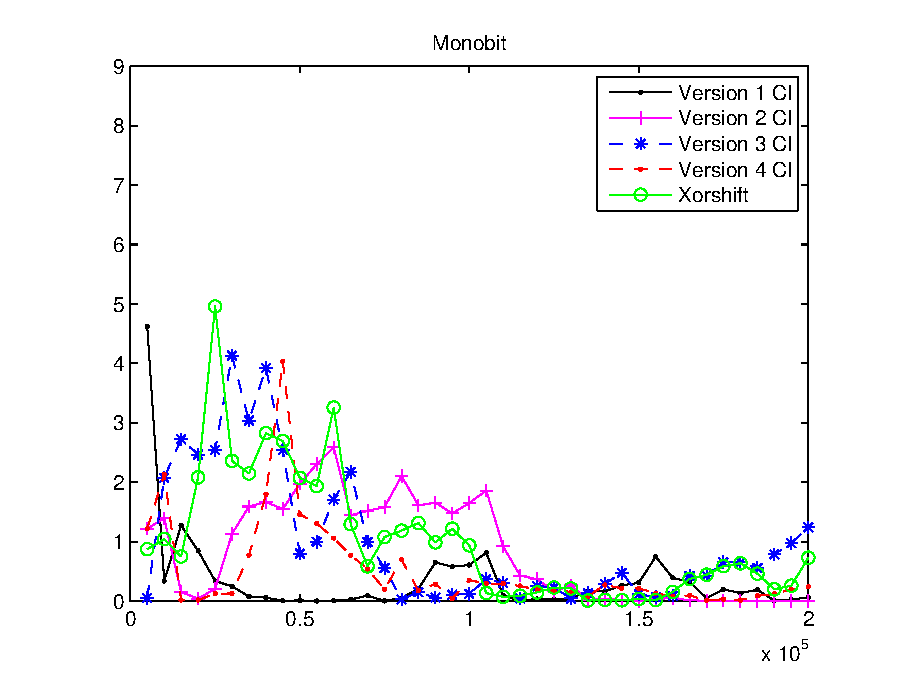
\includegraphics[scale=0.8]{monobits.eps}
% \includegraphics[width=3.7in]{4tests.eps}
\caption{Comparison of monobits tests}
\label{monobits}
\end{figure}

As a comparison of the overall stability of these PRNGs, similar tests have been computed for different sequence lengths (see Fig.\ref{monobits} - Fig.\ref{autocorrelation}).
For the monobit test comparison (Fig.\ref{monobits}), XORshift and CI(XORshift, XORshift) PRNGs versions 2-4 present the same values. They are stable in a low level that never exceeds 1.2. Indeed, the new generators distributes very randomly the zeros and ones, whatever the length of the desired sequence. 
It can also be remarked that the XORshift generator presents the worst performance, but the values are within the standard boundary.
\begin{figure}
\centering
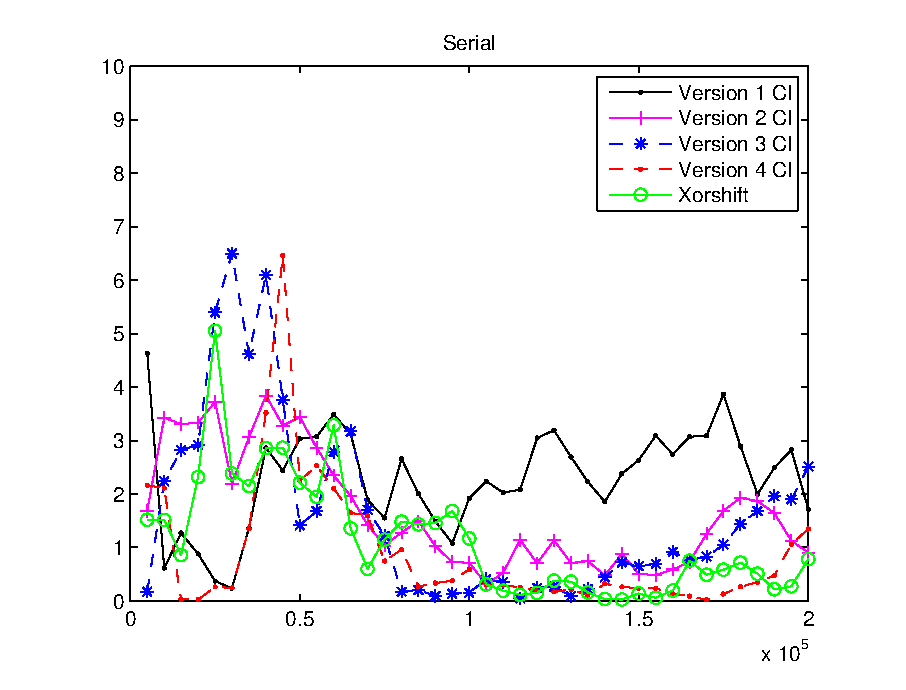
\includegraphics[scale=0.8]{serial.eps}
\caption{Comparison of serial tests}
\label{serial}
\end{figure}

Figure~\ref{serial} shows the serial test comparison. The CIPRNGs outputs outperform this test, for lengths between $2\times 10^4$ and $5 \times 10^4$. 
We can remark too that versions 2 and 3 express a little overflow, even if all generators occurrences of 00, 01, 10, and 11 are very closed to each other.

\begin{figure}
\centering
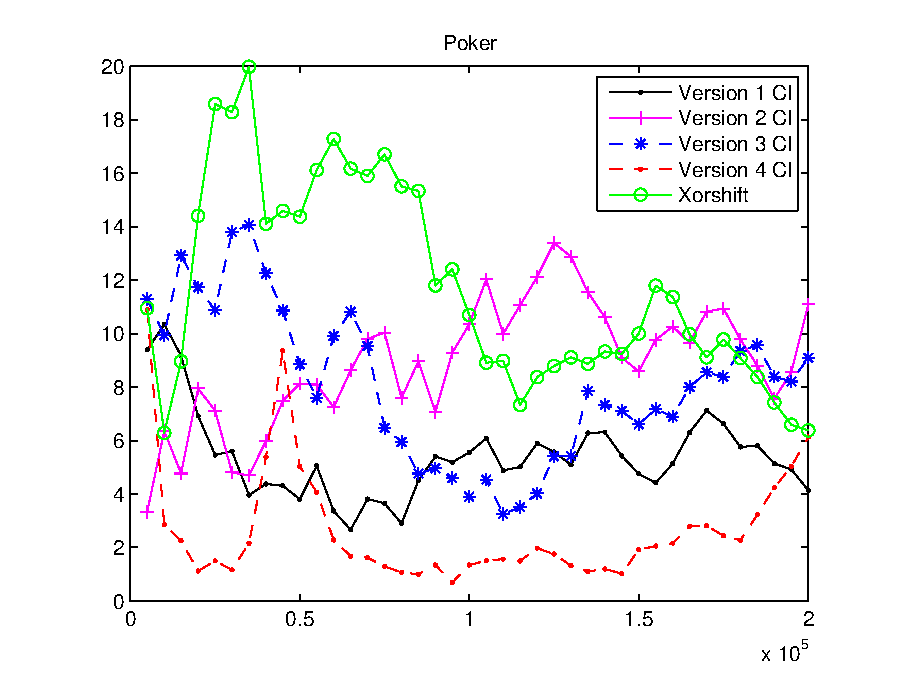
\includegraphics[scale=0.8]{poker.eps}
% \includegraphics[width=3.7in]{4tests.eps}
\caption{Comparison of poker tests}
\label{poker}
\end{figure}

The poker test comparison with $m=8$ is shown in Fig.~\ref{poker}. For some lengths, XORshift is not very stable, whereas 
all the CIPRNGs present good scores (values are lower than the given threshold). 
%The reasons explaining this bad result can be, among other:
Indeed, the value of $m$ and the length of the sequences should be enlarged to be certain that the chaotic iterations express totally their complex behavior. By doing so, the performances of our generators in the poker test can be improved.
%but here we only achieve $2 \times 10^5$ sequence length, then m must be smaller than 13 to comply with the rule, if the sequence length is more, the performance of CI might be better.

\begin{figure}
\centering
% \psfig{figure=2.eps,height=5in,width=3.5in}
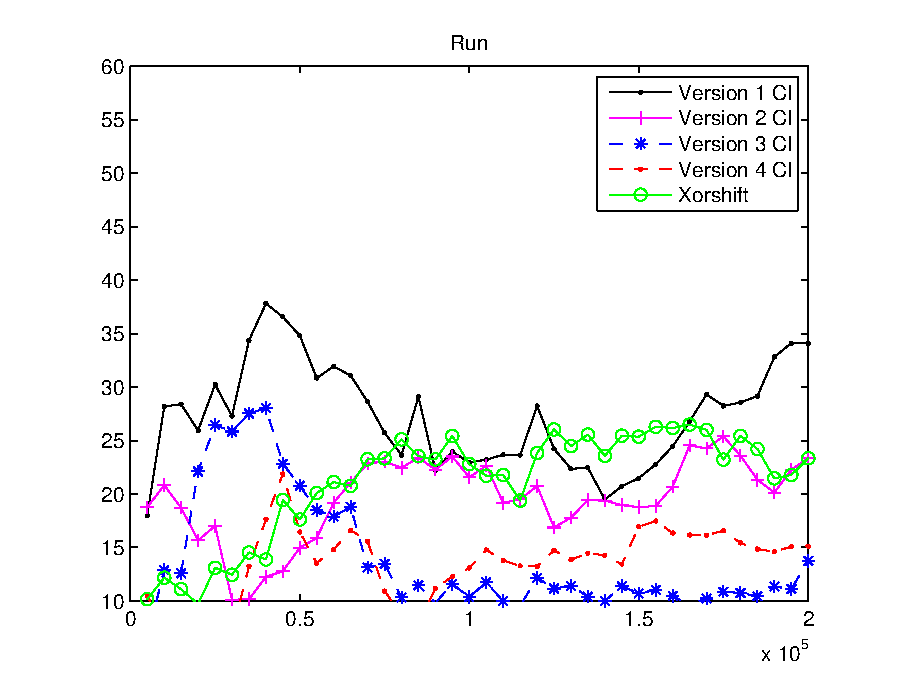
\includegraphics[scale=0.8]{runs.eps}
% \includegraphics[width=3.7in]{4tests.eps}
\caption{Comparison of runs tests}
\label{runs}
\end{figure}

The graphs of the CI generators are the most stable ones during the runs test comparison (Fig.\ref{runs}). Moreover, this trend is reinforced when the lengths of the tested sequences are increased.
%
%
\begin{figure}
\centering
% \psfig{figure=2.eps,height=5in,width=3.5in}
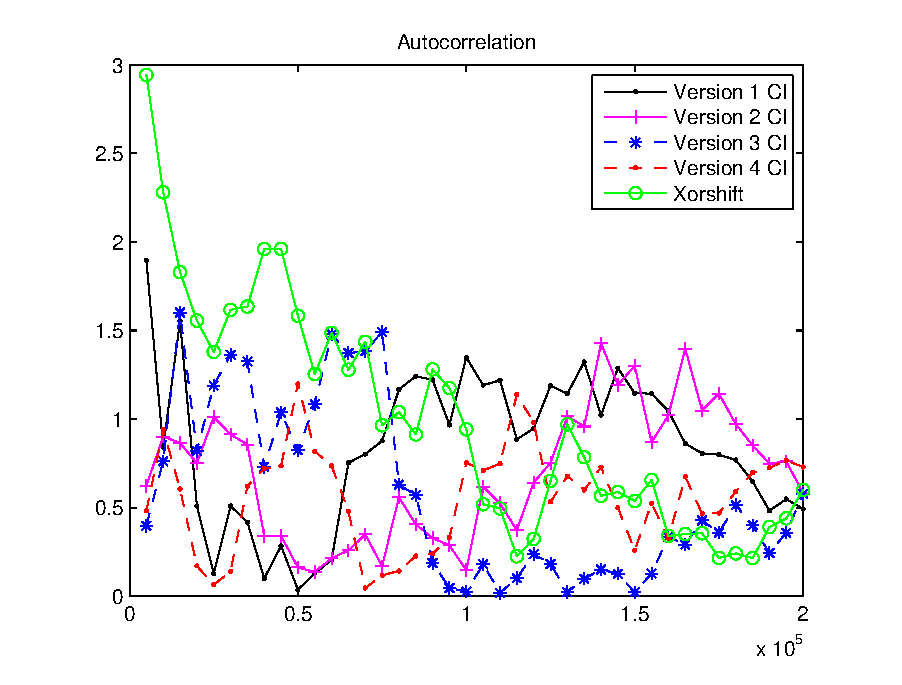
\includegraphics[scale=0.8]{autocorrelation1.eps}
% \includegraphics[width=3.7in]{4tests.eps}
\caption{Comparison of autocorrelation tests}
\label{autocorrelation}
\end{figure}
%
%
The comparison of autocorrelation tests is presented in Fig.~\ref{autocorrelation}. We can see that the CI generators clearly dominate these tests.

As a conclusion of all this study, we can finally claim that the CIPRNGs, whose newer versions run faster than theirs former ones, outperform all of the other generators in these statistical tests, especially when producing long output sequences.



%
%\subsection{A flexible output}
%
%We assume that the initial state $X$ is given as arrays of N-bit integers. Thus, the output size can be flexibly chosenell as $N$. Our PRNGs can generate discrete numbers
%where the number of states could not match to a power of 2, which is suitable for stochastic differential equations as an example.(An attractive property of discrete random numbers is that they
%require a small number of random bits--3 bits)~\cite{Ladd20092140}.
%Moreover, due to the fact that CI process is a simple bitwise change, the speed of output integers and binary numbers is almost the same. 
%
%In the following section, we will discuss the security level for various $N$ by Statistical test.
%For both CI generator, various $N$ can pass all the NIST and DIEHARD test. Table~\ref{TestU01 Statistical Test} gives the results derived from applying the TestU01 battery of tests to the PRNGs considered in this work. As observed,an conclude that the effective range of $N$ for Version 2 CI is bigger than for Version 1 CI by TestU01. And also, this new scheme for obtaining a PRNG by combining two XORshift generators in CI give better properties than the old one (and the individual XORshift alone). It can be observed that the XORshift generator fails 146 tests.
%
%\begin{table}[!t]
%\begin{small}
%\centering
%\renewcommand{\arraystretch}{1.3}
%\caption{TestU01 Statistical Test}
%\label{TestU01 Statistical Test}
%\centering
%\begin{tabular}{cccccccccc}\toprule
%\textbf{CI PRNG}&\textbf{Battery}&\textbf{N=2}&\textbf{N=4}&\textbf{N=8}&\textbf{N=16}&\textbf{N=32} \\\midrule
%
%\multirow{7}*{\textbf{Version 1 CI}}&Rabbit	 	&2	&2	&2	&2	&3 \\
%\multirow{7}*{\textbf{(XORshift,XORshift)}}&Alphabit 				&0	&0	&0	&2	&2 \\
%&Pseudo DieHARD 								&0	&0	&0	&0	&0 \\
%&FIPS\_140\_2 		 							&0	&0	&0	&0	&0 \\
%&Small Crush 		 							&0	&0	&0	&1	&0 \\
%&Crush 		 								&4	&4	&9	&16	&46 \\
%&Big Crush 									&5	&3	&18	&30	&78 \\ 
%\\
%&Number of failures 	 							&11	&9	&29	&51	&129 \\
%\bottomrule
%
%\multirow{7}*{\textbf{Version 2 CI}}&Rabbit 					0	&0	&0	&0	&0 \\
%\multirow{7}*{\textbf{(XORshift,XORshift)}}&Alphabit 				&4	&0	&0	&0	&0 \\
%&Pseudo DieHARD 	 							&8	&2	&0	&0	&0 \\
%&FIPS\_140\_2		 							&2	&0	&0	&0	&0 \\
%&Small Crush 		 							&0	&0	&0	&0	&0 \\
%&Crush 										&0	&0	&0	&0	&0 \\
%&Big Crush 		 							&0	&0	&0	&0	&0 \\ 
%\\
%&Number of failures 	 							&14	&2	&0	&0	&0 \\
%\bottomrule
%\end{tabular}
%\end{small}
%\end{table}
%
%
